%*******************************************************************************
\section[FEBA Model in TRACE]{FEBA Model in TRACE}\label{sec:reflood_feba_trace}
%*******************************************************************************

% Introductory paragraph
The \gls[hyper=false]{feba} facility was modeled using the \gls[hyper=false]{th} system code \gls[hyper=false]{trace}.
The \gls[hyper=false]{trace} code used was a prototypical version developed, with the support of \gls[hyper=false]{usnrc}, for propagation of uncertainties.
The development was a branch from the reference code version \texttt{v5.0 Patch 3} \cite{USNRC2012}.
The model was developed based on specifications provided within the context of the \glsentryshort{premium} benchmark \cite{Skorek2013,Sanz2017},
following whenever possible the modeling best-practices guidelines for the \gls[hyper=false]{trace} code \cite{USNRC2012a} to minimize user's effect.

% TRACE components involved
The model comprised the following \gls[hyper=false]{trace} components:
\marginpar{TRACE components}
\begin{itemize}
	\item A $1$-dimensional \texttt{VESSEL} component to model the bundle test section.
	\item A \texttt{PIPE} component to model upper plenum of the test section.
	\item A \texttt{FILL} component to inlet flow and inlet temperature boundary conditions.
	\item A \texttt{BREAK} component to model the outlet pressure boundary condition.
	\item Two \texttt{HTSTR} components to model the heater rods simulator and non-powered test section housing.
	\item A \textsc{POWER} components to impose electrical power boundary condition.
\end{itemize}

% Nodalization
The \texttt{VESSEL} component was nodalized into $28$ hydraulic nodes of varying sizes between $60$ and $315\,[mm]$.
\marginpar{Model nodalization}
Both the \texttt{HTSTR} components were also nodalized into the same number for the coarse axial conduction nodes.
However, since a large axial temperature gradient was expected in a reflood transient, the fine-mesh reflood flag in \gls[hyper=false]{trace} was enabled.
As a result, each of the course conduction nodes was divided uniformly by $5$, yielding a total of $142$ axial conduction nodes.

The main geometrical parameters and experimental conditions used to develop the \gls[hyper=false]{trace} input model are summarized in Table~\ref{tab:feba_trace}, and the nodalization of the model is illustrated in Fig.~\ref{fig:ch2_feba_nodalization}.

\begin{table}[ht]
    \myfloatalign
    \caption[Geometrical parameters and experimental conditions for the FEBA model in TRACE.]{Geometrical parameters and experimental conditions for the \gls[hyper=false]{feba} model in \gls[hyper=false]{trace}.}
    \label{tab:feba_trace}
    \begin{tabularx}{\textwidth}{Xcc} \toprule
        \tableheadline{Parameter}		  & \tableheadline{Unit} & \tableheadline{Value} \\ \midrule
        Test section total length 		& $[m]$		& $4.114$ \\
        Total heated length 			    & $[m]$		& $3.9$ \\
        Flow area						          & $[m^2]$	& $3.901 \times 10^{-3}$\\
        Hydraulic diameter				    & $[mm]$	& $13.45$\\
        Rectangular housing width   	& $[mm]$	& $78.55$\\
        Rectangular housing thickness	& $[mm]$	& $6.5$\\
        Number of rods					      & $[-]$		& $25$\\
        Rod outer diameter				    & $[mm]$	& $10.75$\\
        Pitch-to-Diameter ratio			  & $[-]$		& $1.33$\\
        Number of spacer grids			  & $[-]$		& $7$\\
        Spacer grid flow obstruction	& $[\%]$	& $20$\\
        \multirow{3}{*}{Spacer grid axial locations}		& \multirow{3}{*}{$[m]$}		& $0.454, 0.999, 1.544,$\\
                                                        &                           & $2.089, 2.634, 3.179,$\\
                                                        &                           & $3.724$ \\
        \midrule
        Number of hydraulic nodes		  & $[-]$		& $28$ (varying length)\\
        \multirow{2}{*}{Number of axial nodes} 	& \multirow{2}{*}{$[-]$}		& $28$ (coarse)\\
                                		  &   		  & $142$ (fine)\\
        \midrule
        Inlet liquid temperature      & $[K]$								&  $312$ \\
        Inlet flow velocity				    & $[cm\cdot s^{-1}]$	& see Table~\ref{tab:feba_exp} \\
        System backpressure           & $[bar]$            	& see Table~\ref{tab:feba_exp} \\
        \bottomrule
    \end{tabularx}
\end{table}

\begin{figure}[bth]
    \centering
    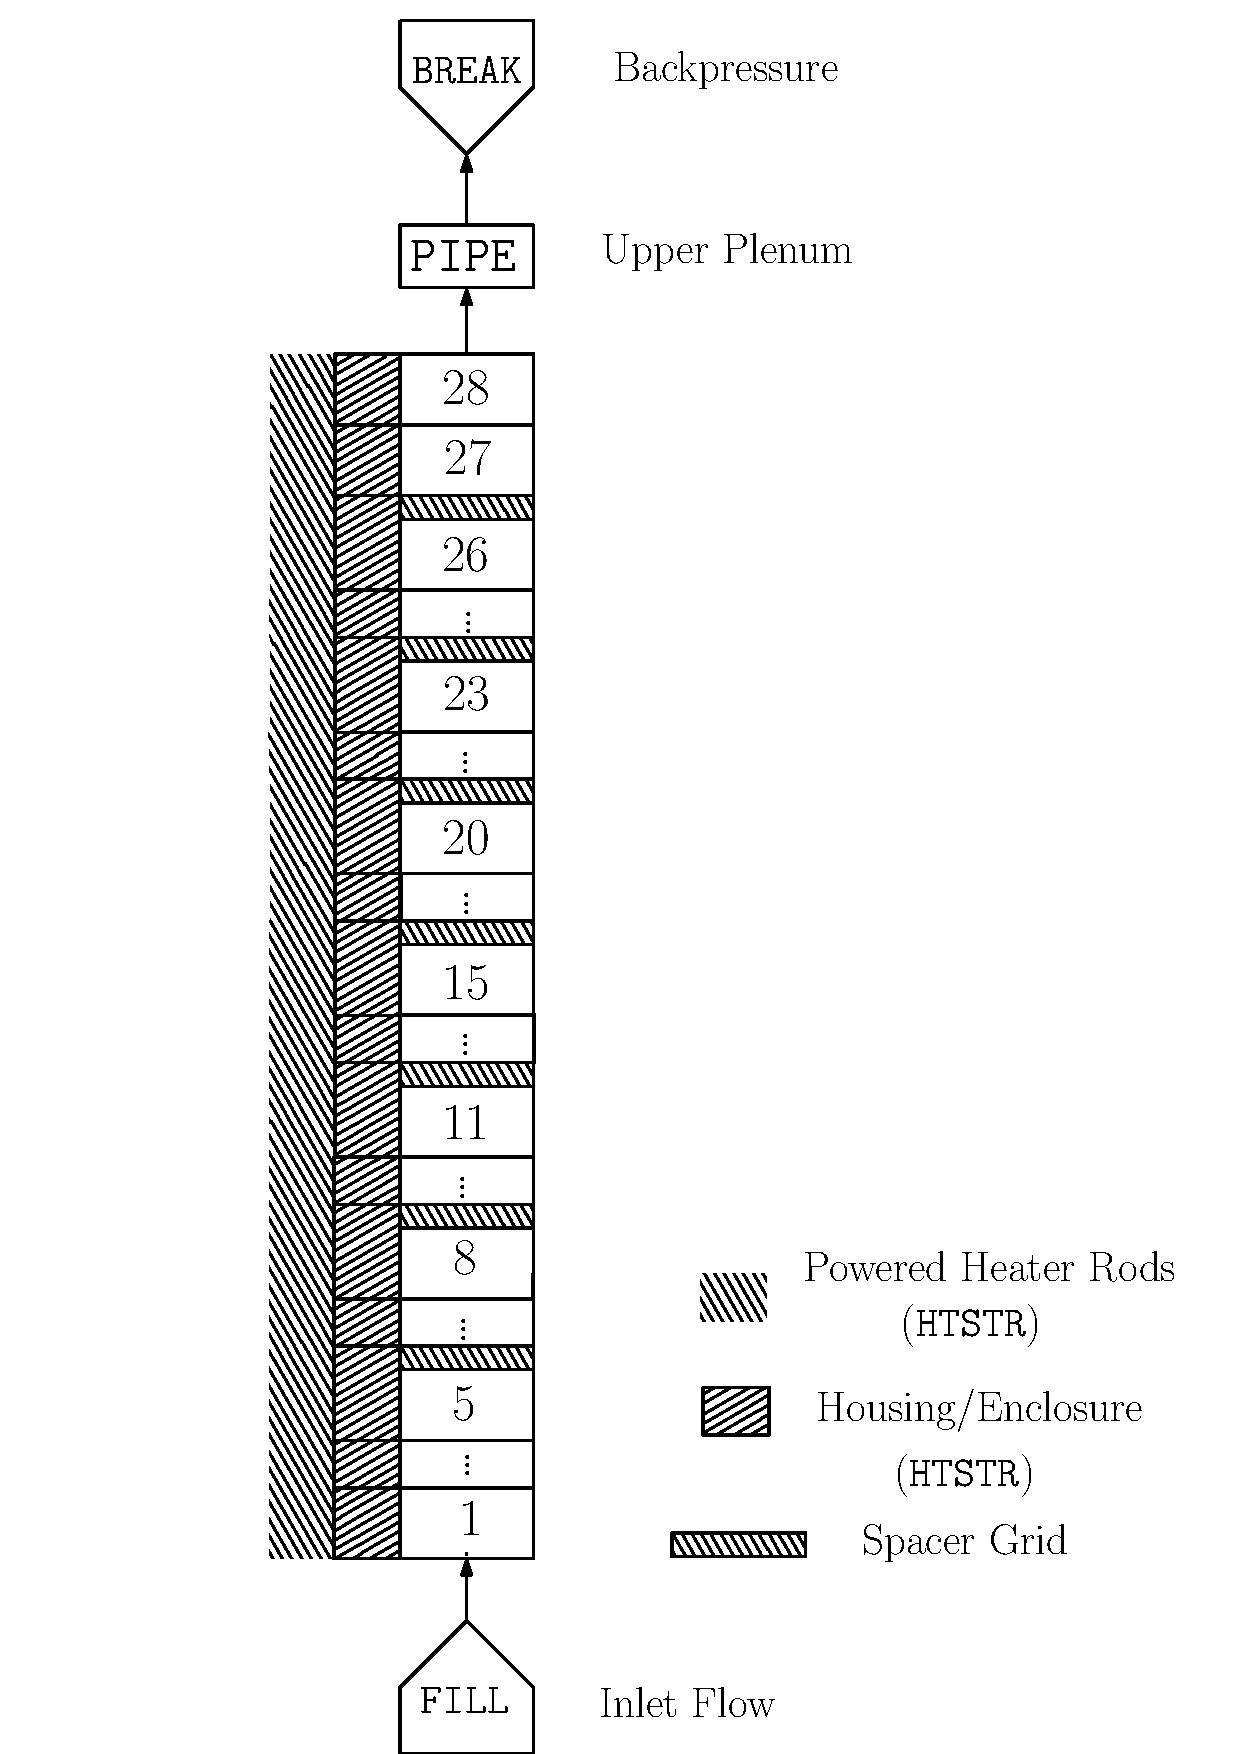
\includegraphics[width=0.65\textwidth]{../figures/chapter2/figures/febaNodalization}
    \caption[Nodalization of the FEBA experimental facility in TRACE.]{Nodalization of the \gls[hyper=false]{feba} experimental facility in \gls[hyper=false]{trace}.}
    \label{fig:ch2_feba_nodalization}
\end{figure}